\ourtool takes as input a set of natural language sentences (from hereon referred to as ``clues'') and (optionally) domain information (names/values of the different entities in the problem domain).
In typical logic grid puzzles, this domain information is present in the grid. 
For some puzzles, domain information is not required; a prototypical example is Einstein's Zebra puzzle, which ends with the question ``who owns the zebra?'', while the puzzle can be solved without knowledge of the fact that there is a zebra in the first place. 
As we will detail below, for some puzzles, especially those with numeric values involved, this domain information is crucial to solving them. 

\ourtool then does this and this and that ... 

Figure \ref{fig:overview} contains an overview of the different components of the system.

\begin{figure*}
\centering
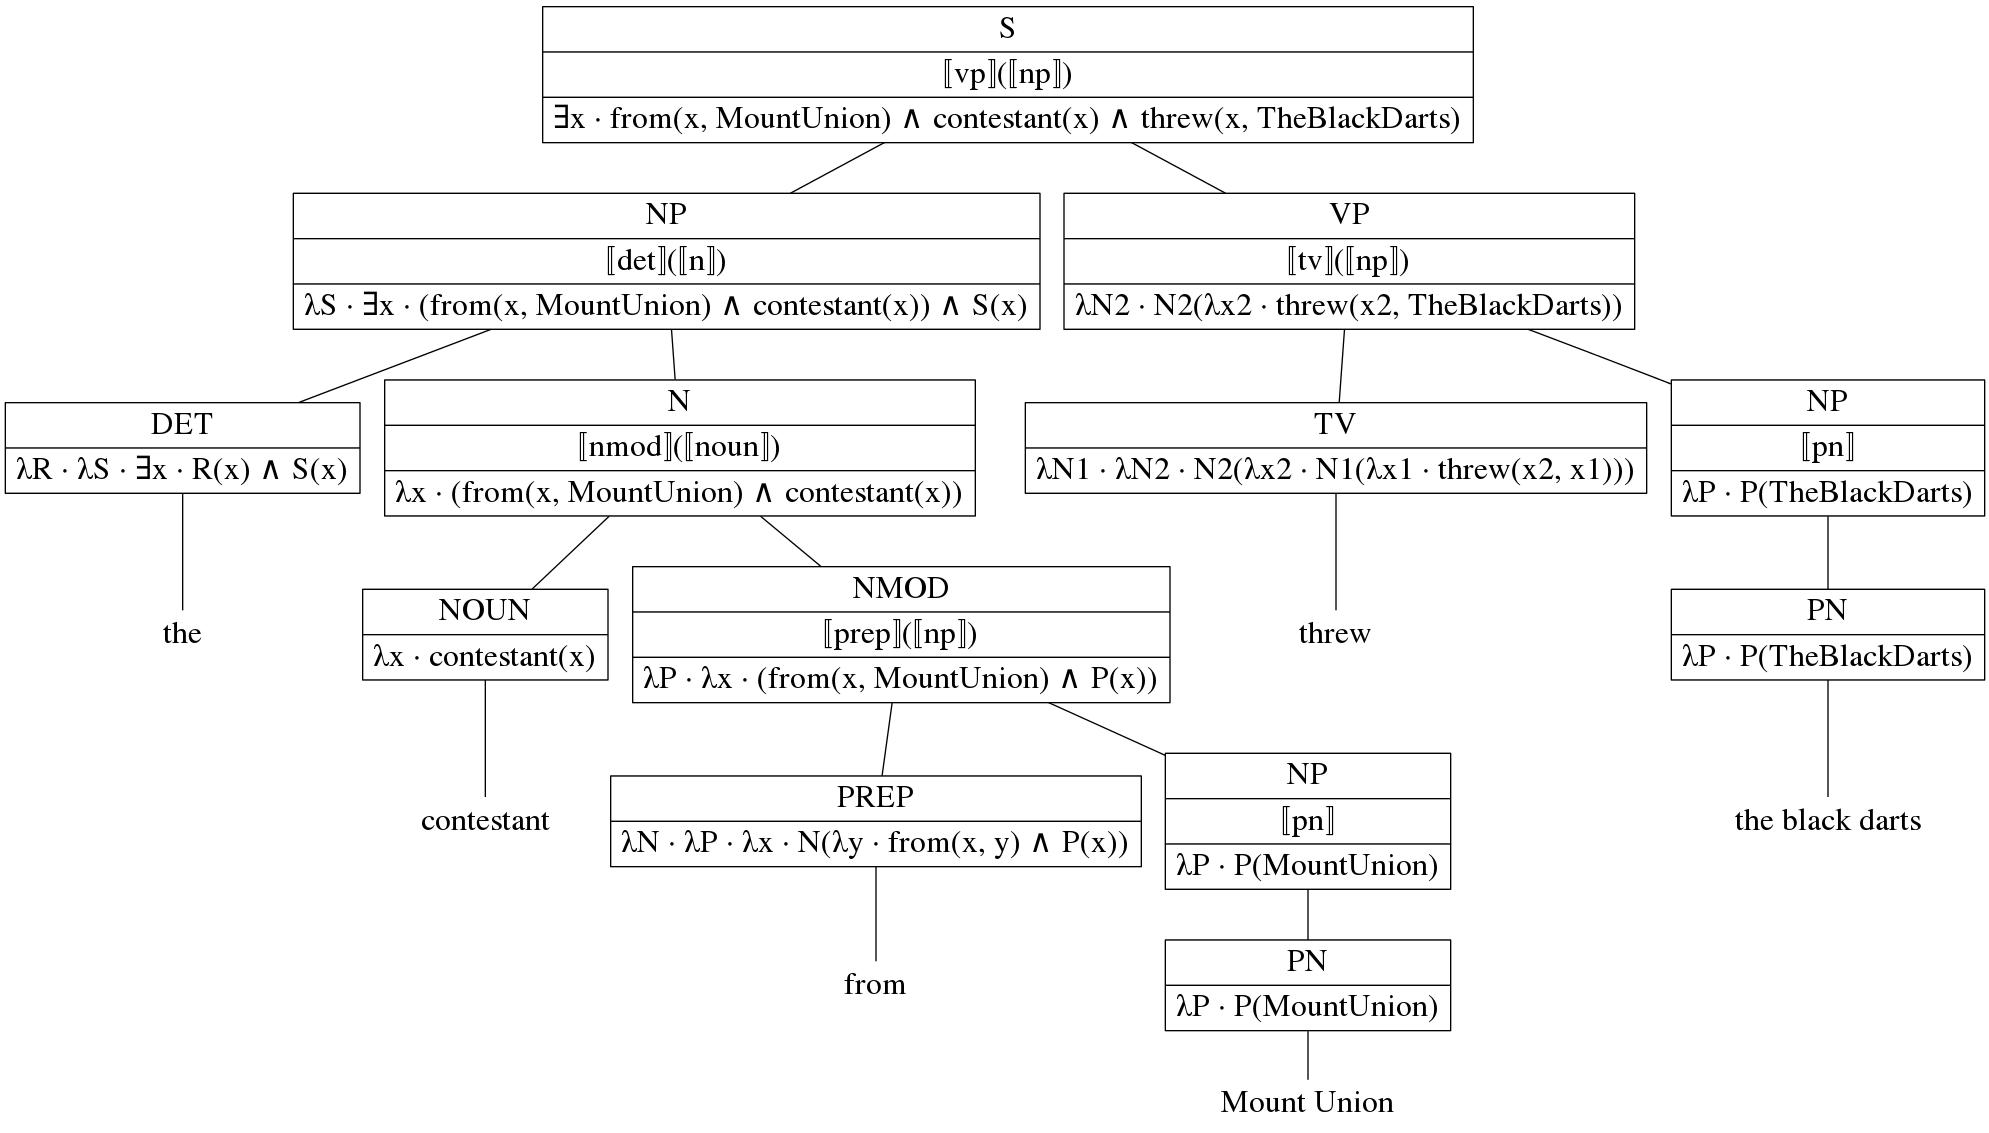
\includegraphics[width=\textwidth]{../../poster/graphviz/tree.jpg}
 Can someone replace this by a picture/schematic overview of the pipeline
 \caption{An overview of the pipeline of \ourtool.}
 \label{fig:overview}
\end{figure*}

